\documentclass[a4paper, 12pt]{article}

%=========
% PACKAGES
%=========

\usepackage{graphicx}
\usepackage[section]{placeins}
\usepackage{float}
\usepackage{amsmath}
\usepackage{listings}
\usepackage{xcolor}
\usepackage{extarrows}
\usepackage{verbatim}
\usepackage{enumerate}
\usepackage{enumitem}
\usepackage{eurosym}
\usepackage{svg}
\usepackage{varwidth}
\usepackage{moreverb}
\usepackage{relsize}
\usepackage{tabto}
\usepackage[margin=1in]{geometry}
\usepackage[normalem]{ulem}
\usepackage{units}
\usepackage{fancyvrb}
\usepackage{fontspec}
\usepackage{extarrows}
\usepackage{amsfonts}
\usepackage{amssymb}
\usepackage{hyperref}
%\usepackage{unicode-math}


%=====================
% SETTINGS/DEFINITIONS
%=====================

% Don't break words with hyphens. Instead, wrap word to next line.
\tolerance=1
% \emergencystretch=\maxdimen
\hyphenpenalty=10000
\hbadness=10000

\definecolor{codegreen}{rgb}{0,0.6,0}
\definecolor{codegray}{rgb}{0.5,0.5,0.5}
\definecolor{codepurple}{rgb}{0.58,0,0.82}
\definecolor{backcolour}{rgb}{0.95,0.95,0.92}

\def\verbatimtabsize{4}

\lstdefinestyle{mystyle}{
	backgroundcolor=\color{backcolour},
	commentstyle=\color{codegreen},
	keywordstyle=\color{magenta},
	numberstyle=\tiny\color{codegray},
	stringstyle=\color{codepurple},
	basicstyle=\ttfamily\footnotesize,
	breakatwhitespace=false,
	breaklines=true,
	captionpos=b,
	keepspaces=true,
	numbers=left,
	numbersep=5pt,
	showspaces=false,
	showstringspaces=false,
	showtabs=false,
	tabsize=2
}

\lstset{style=mystyle}

\setlength{\parindent}{0pt}
\setlength{\parskip}{0em}
\setlength{\jot}{4mm}

\pagenumbering{gobble}

\hypersetup{
    colorlinks=true,
    linkcolor=blue,
    filecolor=blue,      
    urlcolor=blue,
}

\setmainfont{Minion Pro}

\newcommand{\imagesPath}{.}

\title{
	\textbf{Επεξεργασία Φωνής και Φυσικής Γλώσσας} \\~\\
	1η εργαστηριακή άσκηση\\ 
	Εισαγωγή στις γλωσσικές αναπαραστάσεις
}

\author{
	Ηλίας Κουμουκέλης, el18157 \\
	Νικόλαος Παγώνας, el18175
}

\date{}

\begin{document}

\maketitle

\section*{Μέρος 1: Κατασκευή ορθογράφου}
	Στο script \verb|part1.py|, που βρίσκεται στον φάκελο \verb|lab1/|, περιέχεται η υλοποίηση των βημάτων 1-10. Σε αυτό χρησιμοποιούνται ορισμένα από τα αρχεία του φακέλου \verb|scripts/|. Κάποια από τα αρχεία αυτά τα χρησιμοποιήσαμε ως έχουν, ενώ σε κάποια κάναμε μικρές αλλαγές/συμπληρώσεις. \\
	
	Να σημειωθούν τα εξής:
	
	\begin{itemize}
		\item Το \verb|part1.py| υλοποιεί κάποιες χρονοβόρες διαδικασίες, όπως η αξιολόγηση των ορθογράφων και η δημιουργία αρχείου με όλα τα edits. Γι' αυτόν το λόγο, στην πρώτη γραμμή του script ορίζεται η παράμετρος \verb|I_AM_PATIENT|. Όταν έχει την τιμή \verb|False|, οι χρονοβόρες διαδικασίες παραλείπονται, και ο χρόνος εκτέλεσης είναι μερικά δευτερόλεπτα. Αντίθετα, όταν έχει την τιμή \verb|True|, τότε ο χρόνος εκτέλεσης είναι \textasciitilde50 λεπτά (στα δικά μας μηχανήματα). Έτσι μπορεί κάποιος να επιλέξει αν θα εκτελεστούν οι χρονοβόρες διαδικασίες που αναφέρθηκαν. 
		\item Το \verb|part1.py| πρέπει να εκτελεστεί μέσα από τον φάκελο \verb|lab1/|, δηλαδή η εντολή \verb|pwd| πρέπει να τυπώνει: 
		
		\begin{verbatim}
			$ pwd
			
			/path/to/lab1/
		\end{verbatim}
		
		ώστε να μην υπάρξουν θέματα κατά την εύρεση των αρχείων που διαχειρίζεται το \verb|part1.py|.
	\end{itemize} 
	
    \subsection*{Βήμα 1: Κατασκευή corpus}
        \subsubsection*{α)}
        	Αρχικά αφού τρέξαμε το script που κατέβαζει το gutenberg corpus παρατηρήσαμε ότι κάνει μια προεπεξεργασία στα δεδομένα. Συγκεκριμένα:
        	
        	\begin{itemize}
        		\item Απομονώνει κάθε γραμμή του αρχείου ξεχωριστά.
        		\item Αφαιρεί τα επιπλέον κενά, κάνει όλους τους χαρακτήρες lowercase και μετατρέπει φράσεις όπως "\verb|I'm|" στην πλήρη μορφή τους (\verb|"I am"|). 
        		\item Διαγράφει τους χαρακτήρες που δεν είναι γράμματα ή κενά.
        		\item Δημιουργεί έναν πίνακα με στοιχεία τις γραμμές του αρχείου, όπου κάθε γραμμή είναι ένα string
        		\item Αγνοεί τις κενές συμβολοσειρές
        		\item Τέλος γράφει όλα τα στοιχεία του πίνακα που έμειναν από την παραπάνω διαδικασία στο stdout.
        	\end{itemize} 
        	
        	Μία περίπτωση στην οποία θα θέλαμε να διατηρήσουμε τα σημεία στίξης είναι αν θέλουμε να διορθώσουμε αρκτικόλεξα, οπότε εκεί δεν θα επιθυμούσαμε τόσο επιθετικό preprocessing.
        	
        \subsubsection*{β)}
        	Με την επέκταση του corpus: 
        	
        	\begin{itemize}
        		\item Εμπλουτίζουμε το data set μας με περισσότερα στοιχεία (λέξεις, ιδιωματισμούς, ορολογίες κλπ.) από άλλες περιοχές. Έτσι για παράδειγμα, το corpus μπορεί να συμπεριλάβει και λέξεις που συναντώνται συχνά σε συγκεκριμένα γνωστικά αντικείμενα, αλλά είναι σπάνιες εκτός αυτών.
        		\item Μεγαλώνει ο δειγματικός χώρος και επομένως αυξάνεται η δυνατότητα κατάταξης της συχνότητας εμφάνισης των λέξεων, διορθώνοντας πιθανές ανωμαλίες. Για παράδειγμα, ένα βιβλίο όπως ο Tom Sawyer θα περιλαμβάνει πολλές φορές την λέξη "Tom", όμως αν συμπεριλάβουμε μεγάλο αριθμό βιβλίων, η συχνότητα εμφάνισης της λέξης "Tom" σταματά να είναι τόσο έντονη σε σχέση με άλλες λέξεις που είναι συχνές σε όλα τα βιβλία, όπως η λέξη "the".
        	\end{itemize} 
        
    \subsection*{Βήμα 2: Κατασκευή λεξικού}
        \subsubsection*{α)}
        	Δημιουργούμε ένα dictionary της μορφής \verb|{token: number of occurrences}|

        \subsubsection*{β)}
        	Φιλτράρουμε το λεξικό, απορρίπτοντας τις λέξεις που έχουν εμφανιστεί κάτω από 5 φορές. Αυτό το βήμα χρειάζεται, διότι αλλιώς το FST που θα φτιάχναμε θα λάμβανε υπόψιν του πάρα πολλές λέξεις με αποτέλεσμα τόσο ο αποθηκευτικός χώρος που χρειάζεται το FST, όσο και ο χρόνος που απαιτούν πράξεις όπως η βελτιστοποίηση του FST και η διόρθωση μιας λέξης θα αύξαναν απαγορευτικά, ειδικά αν αναλογιστούμε το πόσο μικρό όφελος προσφέρουν τόσο σπάνιες λέξεις που κατά πάσα πιθανότητα δεν θα προτιμηθούν ποτέ από τον ορθογράφο μας.
        	
        \subsubsection*{γ)}
        	Αποθηκεύουμε το λεξικό που φτιάξαμε στο αρχείο \verb|vocab/words.vocab.txt| σε δύο tab separated στήλες, όπου η πρώτη στήλη περιέχει τα tokens και η δεύτερη στήλη τους αντίστοιχους αριθμούς εμφανίσεων.
    
    \subsection*{Βήμα 3: Δημιουργία συμβόλων εισόδου/εξόδου}
        \subsubsection*{α)}
        	Δημιουργούμε το αρχείο \verb|vocab/chars.syms| στο οποίο αποθηκεύουμε στην πρώτη στήλη το κάθε γράμμα και στην δεύτερη έναν αύξοντα ακέραιο αριθμό-index (το \verb|<eps>| αντιστοιχεί στο 0 και οι υπόλοιποι χαρακτήρες αντιστοιχούν στον ASCII κωδικό τους), με τη βοήθεια των συναρτήσεων \verb|lowercase_to_index()| και \verb|create_lowercase_to_index_file()|.
        \subsubsection*{β)} 
        	Αντίστοιχα κάνουμε το ίδιο για τα tokens με τη βοήθεια της συνάρτησης \verb|create_word_to_index_file()|, και αποθηκεύουμε το αποτέλεσμα στο αρχείο \verb|vocab/words.syms|. Να σημειωθεί ότι και εδώ χρειάζεται το \verb|<eps>| να αντιστοιχεί στο 0. 
    
    \subsection*{Βήμα 4: Κατασκευή μετατροπέα edit distance}
        \subsubsection*{α)}
        	Φτιάχνουμε έναν μετατροπέα $L$ βασισμένο στην απόσταση Levenshtein με τη βοήθεια της συνάρτησης \verb|create_L_transducer_file()|. Κάθε μετατροπή χαρακτήρα έχει το αντίστοιχο κόστος:
            
            \paragraph*{1)}
            	Κάθε χαρακτήρας αντιστοιχίζεται στον εαυτό του με βάρος 0 \textbf{(καμία αλλαγή)}.
            	
            \paragraph*{2)}
            	Κάθε χαρακτήρας αντιστοιχίζεται στο \verb|<eps>| με βάρος 1 \textbf{(διαγραφή)}.
            
            \paragraph*{3)}
            	Το \verb|<eps>| αντιστοιχίζεται σε κάθε χαρακτήρα με βάρος 1 \textbf{(εισαγωγή)}.
            
            \paragraph*{4)}
            	Κάθε χαρακτήρας αντιστοιχίζεται σε κάθε άλλο χαρακτήρα με βάρος 1. \\
        
        Αν πάρουμε το shortest path, αυτός ο μετατροπέας θα παράγει τις λέξεις στις οποίες μετασχηματίζεται η λέξη εισόδου, με το μονοπάτι μετασχηματισμών να έχει ελάχιστο κόστος, δηλαδή θα αφήσει την λέξη απαράλλαχτη με κόστος 0. 
        
        \subsubsection*{β)}
        	Η συνάρτηση \verb|create_L_transducer_file()| αναλαμβάνει και την αποθήκευση του αρχείου \verb|fsts/L.fst|.
        	
        \subsubsection*{γ)}
        	Με την βοήθεια της \verb|fstcompile| δημιουργούμε το αρχείο \verb|fsts/L.binfst|. 
        
        \subsubsection*{δ)}
        	Πιθανά edits που θα μπορούσαμε να συμπεριλάβουμε είναι:
        	
        	\begin{itemize}
        		\item Να λάβουμε υπόψιν λάθη που κάνουν συχνά άτομα με δυσλεξία (πχ 3 $\rightarrow$ ε). Αυτό φυσικά προϋποθέτει να έχουμε συμπεριλάβει χαρακτήρες όπως το 3 και το ε.
        		\item Να λάβουμε υπόψιν edits της μορφής \verb|r| $\rightarrow$ \verb|rr| (πχ στη λέξη occurrence)
        	\end{itemize}
        	
        \subsubsection*{ε)}
			Επειδή ορισμένα πλήκτρα στο πληκτρολόγιο είναι πιο κοντά μεταξύ τους, μπορούμε να τροποποιήσουμε τα βάρη έτσι ώστε τα edits που αφορούν κοντινά πλήκτρα να προτιμώνται έναντι αυτών που τα πλήκτρα είναι μακρύτερα. (πχ το \verb|q| και το \verb|w| είναι πολύ κοντύτερα απ' ό,τι το \verb|q| και το \verb|p|, επομένως είναι λογικό το edit \verb|q| $\rightarrow$ \verb|w| να κοστίζει λιγότερο απ' ό,τι το edit \verb|q| $\rightarrow$ \verb|p|) 

        	
        \subsubsection*{ζ)}
			Χρησιμοποιούμε την \verb|fstdraw| για να σχεδιάσουμε τον $L$. Χρησιμοποιούμε ένα πολύ μικρό υποσύνολο των χαρακτήρων για εύκολη οπτικοποίηση.
			

			\begin{figure}[H]
				\begin{center}
					\includegraphics[width=0.15\linewidth]{\imagesPath/lab1/fsts/L_small_handcrafted.png}
				\end{center}
			\end{figure}
			

			    
    \subsection*{Βήμα 5: Κατασκευή αποδοχέα λεξικού}
        \subsubsection*{α)}
        	Με τη χρήση της συνάρτησης \verb|create_V_acceptor_file()| κατασκευάζουμε έναν αποδοχέα $V$ με μία αρχική κατάσταση και μηδενικά βάρη στις ακμές του. Αυτός ο αποδοχέας απλά αποδέχεται μια λέξη αν αυτή ανήκει στο λεξικό.
        	 
        \subsubsection*{β)}
        	Καλούμε τις \verb|fstrmepsilon|, \verb|fstdeterminize| και \verb|fstminimize| ώστε να βελτιστοποιήσουμε το μοντέλο. Οι εντολές αυτές εκτελούν τις ακόλουθες πράξεις (κάθε φορά το FST που προκύπτει είναι ισοδύναμο):
        	
        	\begin{itemize}
        		\item \verb|fstrmepsilon|: Αφαιρεί τις ε-μεταβάσεις (όπου είσοδος και έξοδος είναι ε). 
        		\item \verb|fstdeterminize|: Κάνει ντετερμινιστικό τον transducer, δηλαδή καμία κατάσταση δεν έχει δύο μεταβάσεις με την ίδια είσοδο.
        		\item \verb|fstminimize|: Ελαχιστοποιεί τον transducer, δηλαδή φτιάχνει ένα ισοδύναμο transducer με τον ελάχιστο δυνατό αριθμό καταστάσεων.
        	\end{itemize}
        	
        \subsubsection*{γ)}
        	Αποθηκεύουμε το αρχείο σε Openfst text format με όνομα \verb|fsts/V.fst|.
        	
        \subsubsection*{δ)}
        	Με την \verb|fstcompile| κάνουμε compile τον αποδοχέα και δημιουργούμε το αρχείο \verb|fsts/V.binfst|.
        	
        \subsubsection*{ε)}
        	Χρησιμοποιούμε την \verb|fstdraw| για να σχεδιάσουμε τον $V$, χρησιμοποιώντας ένα μικρό υποσύνολο των λέξεων για εύκολη οπτικοποίηση. Συγκεκριμένα, σχεδιάζουμε:
        	
        	\begin{itemize}
        		\item Τον $V$ πριν εφαρμοστεί οποιαδήποτε βελτιστοποίηση:
        			\begin{figure}[H]
        				\includegraphics[width=\linewidth]{\imagesPath/lab1/fsts/V_nonoptimal_small.png}
        			\end{figure}
				\item Ύστερα από την \verb|fstrmepsilon|:
					\begin{figure}[H]
						\includegraphics[width=\linewidth]{\imagesPath/lab1/fsts/V_rmepsilon_small.png}
					\end{figure}
				\item Ύστερα και από την \verb|fstdeterminize| (δεν υπάρχει κάποια αλλαγή):
					\begin{figure}[H]
						\includegraphics[width=\linewidth]{\imagesPath/lab1/fsts/V_rmepsilon_determinized_small.png}
					\end{figure}
				\item Τέλος, ύστερα και από την \verb|fstminimize|:
					\begin{figure}[H]
						\includegraphics[width=\linewidth]{\imagesPath/lab1/fsts/V_optimal_small.png}
					\end{figure}
        	\end{itemize}
        
    \subsection*{Βήμα 6: Κατασκευή ορθογράφου}
        \subsubsection*{α)}
        	Συνθέτουμε τον $L$ με τον $V$, παράγοντας έναν edit distance spell checker $S$, ο οποίος  λειτουργεί με μοναδικό κριτήριο να ελαχιστοποιήσει το κόστος των edits που χρειάζονται ώστε μία λανθασμένη λέξη να μετατραπεί σε μία σωστή (που ανήκει δηλαδή στο λεξικό). Φροντίζουμε να καλέσουμε την \verb|fstarcsort| στις εξόδους του $L$ και στις εισόδους του $V$ ώστε να μην υπάρξουν προβλήματα κατά τη σύνθεση. 
        	
            \paragraph{1)}
            	Στην περίπτωση που τα edits είναι ισοβαρή, ουσιαστικά ο transducer έχει ως σκοπό να κάνει το μικρότερο πλήθος edits ώστε να φτάσει σε μία έγκυρη λέξη.
            \paragraph{2)}
            	Στην περίπτωση που τα edits έχουν διαφορετικά βάρη, μπορούμε να εισάγουμε περισσότερη "ευφυΐα" στον μετατροπέα, δίνοντας μικρότερο βάρος σε πιθανότερες διορθώσεις, ώστε να προτιμηθούν. 
            	
        \subsubsection*{β)}
    		Πιθανές προβλέψεις του min edit spell checker:
    		
    		\begin{itemize}
    			\item \verb|cit| $\rightarrow$ \verb|cat| (1 αλλαγή), \verb|it| (1 διαγραφή), \verb|cite| (1 προσθήκη)
    			\item \verb|cwt| $\rightarrow$ \verb|cut|, \verb|cat| (1 αλλαγή)
    		\end{itemize}
    		
    \subsection*{Βήμα 7: Δοκιμή ορθογράφου}
        \subsubsection*{α)}
        	Χρησιμοποιούμε το \verb|lab1/data/spell_test.txt| για το evaluation.
        \subsubsection*{β)}
        	Χρησιμοποιούμε τη συνάρτηση \verb|test_spell_checker()| η οποία καλεί το \verb|lab1/scripts/predict.sh| για τις 20 πρώτες λέξεις του test set. Ενδεικτικά:
        	
        	\begin{verbatim}
        	    	Wrong word      Corrected word      Actual word
        		------------------|------------------|--------------------
        		contenpted        |  contented       |   contented
        		contende          |  contend         |   contented
        		begining          |  beginning       |   beginning
        		problam           |  problem         |   problem
        		proble            |  problem         |   problem
        		dirven            |  driven          |   driven
        		exstacy           |  exactly         |   ecstasy
        		ecstacy           |  ecstasy         |   ecstasy
        		guic              |  guil            |   juice
        		juce              |  juice           |   juice
        		localy            |  local           |   locally
        		compair           |  compare         |   compare
        		pronounciation    |  pronouncing     |   pronunciation
        		transportibility  |  respectability  |   transportability
        		miniscule         |  mince           |   minuscule
        	\end{verbatim}
        	
        	Όσον αφορά το \verb|predict.sh|, αυτό δημιουργεί με τη χρήση του \verb|mkfstinput.py| ένα FST που αποδέχεται τη λανθασμένη λέξη εισόδου και το συνθέτει με τον spell checker. Βρίσκει το shortest path στη σύνθεση αυτή και αφαιρεί τις ε-μεταβάσεις. Η fstprint τυπώνει τις καταστάσεις που περιλαμβάνει το shortest path μαζί με την έξοδό τους, οπότε επιλέγοντας μόνο τις εξόδους (με την εντολή cut) και ύστερα φιλτράροντας ε-εξόδους και την γραμμή της τελικής κατάστασης, μένει μόνο η λέξη εξόδου, που είναι και η διορθωμένη.
        
    \subsection*{Βήμα 8: Υπολογισμός κόστους των edits}
        Σε αυτό το βήμα χρησιμοποιούμε το corpus \verb|lab1/data/wiki.txt| που περιέχει συχνά ορθογραφικά λάθη της Wikipedia, προκειμένου να δώσουμε διαφορετικό κόστος σε κάθε edit operation. Να σημειωθεί ότι διαγράψαμε 3 γραμμές από το \verb|wiki.txt| οι οποίες περιείχαν χαρακτήρες που δεν ήταν πεζά αγγλικά γράμματα (π.χ. \verb|a.k.a.|). Τρέχουμε το \verb|scripts/word_edits.sh| που εκτελεί τα βήματα (α), (β) και (γ):
        
        \subsubsection*{α)}   
        	Αρχικά χρησιμοποιούμε ένα μόνο παράδειγμα (abandonned $\rightarrow$ abandoned). Δημιουργούμε έναν αποδοχέα $M$ για τη λανθασμένη λέξη (abandonned) και ένα μετατροπέα $N$ για τη διορθωμένη (abandoned).
        	
        \subsubsection*{β)}   
        	Δημιουργούμε τη σύνθεση $MLN$.
        	
        \subsubsection*{γ)}   
        	Εκτελούμε την \verb|fstshortestpath| ακολουθούμενη από την \verb|fstprint| με την σύνταξη που ζητείται, παράγοντας ένα μονοπάτι ελάχιστου κόστους για τη διόρθωση της λανθασμένης λέξης. Με την \verb|grep| αγνοούμε τις γραμμές με μηδενικό κόστος και με την \verb|cut| επιλέγουμε μόνο τα edits. 
        	
        	Εν συντομία, το \verb|word_edits.sh| (με τη βοήθεια του \verb|mkfstinput.py|):
        	
        	\begin{itemize}
        		\item Δημιουργεί ένα FST $M$ που αποδέχεται τη λανθασμένη λέξη 
        		\item Δημιουργεί ένα FST $N$ που αποδέχεται τη σωστή λέξη
        		\item Συνθέτει το $M$ με τον $L$ και στη συνέχεια με το $N$, παράγοντας το $MLN$
        		\item Βρίσκει το shortest path πάνω στο $MLN$
        		\item Φιλτράρει κατάλληλα (με τις εντολές grep και cut) την έξοδο της \verb|fstprint| πάνω στο $MLN$ ώστε να μείνουν μόνο τα edits μη μηδενικού κόστους.
        	\end{itemize}
        	
        	Παραδείγματα εκτέλεσης:
        	
        	\begin{verbatim}
        		$ bash scripts/word_edits.sh helo hello
        		<eps>     l
        		
        		$ bash scripts/word_edits.sh mrlow mellow
        		r         l 
        		<eps>     e
        		
        		$ bash scripts/word_edits.sh crase increase
        		<eps>     i 
        		<eps>     e
        		<eps>     n
        	\end{verbatim}
        
        \subsubsection*{δ)}
        	Γράφουμε τη συνάρτηση \verb|save_all_edits_to_file()| η οποία εκτελεί την παραπάνω διαδικασία για κάθε ζεύγος λέξεων στο \verb|wiki.txt| και αποθηκεύει όλα τα edits στο αρχείο \verb|lab1/data/edits.txt|.
        	
        \subsubsection*{ε)}   
        	Εξάγουμε τη συχνότητα κάθε edit με την συνάρτηση \verb|extract_frequency_to_dict()| και την αποθηκεύουμε σε ένα λεξικό στη μορφή:
        	
        	\begin{verbatim}
				{(source, target): frequency}
        	\end{verbatim}
        
        \subsubsection*{στ)}   
        	Επαναλαμβάνουμε το βήμα 4, όπου κατασκευάζουμε τον μετατροπέα edit distance, αλλά αυτή τη φορά τα edits έχουν διαφορετικό κόστος μεταξύ τους. Συγκεκριμένα, κάθε edit έχει βάρος ίσο με:
        	
        	\[
        		-\log\left(\text{frequency}\right) = -\log\left(\frac{\text{number of occurrences for the particular edit}}{\text{total number of edits}}\right)
        	\]
        	
        	Αν κάποιο edit δεν έχει εμφανιστεί στο corpus βάζουμε έναν πολύ μεγάλο αριθμό ως βάρος (σταθερά \verb|INFINITY|). Έτσι προκύπτει ο transducer $E$.
        
        \subsubsection*{ζ)}
        	Επαναλαμβάνουμε τα βήματα 6, 7 χρησιμοποιώντας τον transducer $E$ αντί για τον $L$, δηλαδή κατασκευάζουμε και δοκιμάζουμε τον ορθογράφο $EV$.
        	
        	Ενδεικτικά:
        	
        \begin{verbatim}
			    Wrong word      Corrected word      Actual word
			------------------|------------------|--------------------
			contenpted        |  contented       |   contented
			contende          |  contend         |   contented
			begining          |  beginning       |   beginning
			problam           |  problem         |   problem
			proble            |  problem         |   problem
			dirven            |  driven          |   driven
			exstacy           |  exactly         |   ecstasy
			ecstacy           |  ecstasy         |   ecstasy
			guic              |  guil            |   juice
			juce              |  juice           |   juice
			localy            |  local           |   locally
			compair           |  compare         |   compare
			pronounciation    |  pronouncing     |   pronunciation
			transportibility  |  respectability  |   transportability
			miniscule         |  mince           |   minuscule
         \end{verbatim}
    
    \subsection*{Βήμα 9: Εισαγωγή της συχνότητας εμφάνισης λέξεων (Unigram word model)}
    	Σε αυτό το βήμα σκοπός είναι να εκμεταλλευτούμε την συχνότητα εμφάνισης των λέξεων, ώστε ο ορθογράφος να προτιμά πιο συχνές λέξεις ως πιο πιθανές. 
    
        \subsubsection*{α)}
        	Χρησιμοποιούμε το λεξικό συχνοτήτων που φτιάξαμε στο Βήμα 2.
        	   
        \subsubsection*{β)}   
        	Κατασκευάζουμε τον αποδοχέα $W$ που έχει μία κατάσταση και αντιστοιχίζει κάθε λέξη στον εαυτό της με βάρος ίσο με $-\log(\text{frequency})$, όπου frequency είναι η (σχετική) συχνότητα εμφάνισης της αντίστοιχης λέξης.
        	
        \subsubsection*{γ)}   
        	Κατασκευάζουμε τον ορθογράφο $LVW$ συνθέτοντας τον $L$ με τον $V$ και ύστερα με το $W$. Κάνουμε optimize τον $W$ (οι $L$ και $V$ είναι ήδη optimized) με χρήση των \verb|fstrmepsilon|, \verb|fstdeterminize| και \verb|fstminimize|. Για την σύνθεση χρησιμοποιούμε την \verb|fstarcsort| στις εξόδους του αριστερού μέρους και στις εισόδους του δεξιού.
        	
        
        \subsubsection*{δ)}   
        	Με παρόμοιο τρόπο κατασκευάζουμε τον ορθογράφο $EVW$.
        	
        \subsubsection*{ε)}
        	Αξιολογούμε τον ορθογράφο $LVW$ με την διαδικασία του ερωτήματος 8, και αναφέρουμε ενδεικτικά κάποιες διορθώσεις:
        	
        	\begin{verbatim}
        		  	Wrong word      Corrected word      Actual word
	      		------------------|------------------|--------------------
	      		contenpted        |  the             |   contented
	      		contende          |  the             |   contented
	      		begining          |  beginning       |   beginning
	      		problam           |  of              |   problem
	      		proble            |  the             |   problem
	      		dirven            |  the             |   driven
	      		exstacy           |  the             |   ecstasy
	      		ecstacy           |  the             |   ecstasy
	      		guic              |  the             |   juice
	      		juce              |  the             |   juice
	      		localy            |  and             |   locally
	      		compair           |  and             |   compare
	      		pronounciation    |  unto            |   pronunciation
	      		transportibility  |  and             |   transportability
	      		miniscule         |  the             |   minuscule
        	\end{verbatim}
        	
        	Βλέπουμε ότι σχεδόν όλες οι λέξεις έχουν μετατραπεί σε "the" και "and", ακριβώς επειδή αυτές οι λέξεις είναι πολύ συχνές και υπερνικούν όλα τα άλλα πιθανά μονοπάτια, οδηγώντας σε πολύ χειρότερη επίδοση του ορθογράφου.
        	   
        \subsubsection*{στ)}   
        	Συγκρίνουμε τα αποτελέσματα του $LVW$ με τον $LV$. Η έξοδος των μετατροπέων σε κάθε περίπτωση είναι:
        	
        	\begin{itemize}
        		\item $LVW$:
        			\begin{itemize}
        				\item \verb|cwt| $\rightarrow$ \verb|the|
        				\item \verb|cit| $\rightarrow$ \verb|it|
        			\end{itemize}
        		\item $LV$:
        			\begin{itemize}
        				\item \verb|cwt| $\rightarrow$ \verb|cut|
        				\item \verb|cit| $\rightarrow$ \verb|city|
        			\end{itemize}
        	\end{itemize}
        	
        	Βλέπουμε ότι ο $LVW$ δείχνει ισχυρή προτίμηση σε συχνά εμφανιζόμενες λέξεις, ακόμα κι αν δεν έχουν καμία σχέση με την είσοδο (π.χ. \verb|cwt| $\rightarrow$ \verb|the|). Αντίθετα, ο $LV$ απλώς προσπαθεί να φτάσει σε μία έγκυρη λέξη με τον μικρότερο αριθμό edits.
        
        \subsubsection*{ζ)}  
        	Χρησιμοποιούμε την \verb|fstdraw| για να σχεδιάσουμε τον $W$ και τον $VW$. Χρησιμοποιούμε ένα μικρό υποσύνολο των λέξεων για πιο εύκολη οπτικοποίηση.
        	
        	\begin{figure}[H]
        		\includegraphics[width=0.3\linewidth]{\imagesPath/lab1/fsts/W.png}
        	\end{figure}
        	
        	\begin{figure}[H]
        		\includegraphics[width=\linewidth]{\imagesPath/lab1/fsts/VW.png}
        	\end{figure}
        
    \subsection*{Βήμα 10: Αξιολόγηση των ορθογράφων}
    	Χρησιμοποιούμε το \verb|run_evaluation.py| για να συγκρίνουμε τα αποτελέσματα των ορθογράφων ~ $LV, LVW, EV, EVW$. Ως test set χρησιμοποιούμε το αρχείο \verb|data/spell_test.txt|. Έχουμε:
    	
    	\begin{itemize}
    		\item $LV$ accuracy: \textasciitilde0.596 = 59.6\%
    		\item $LVW$ accuracy: \textasciitilde0.044 = 4.4\%
    		\item $EV$ accuracy: \textasciitilde0.689 = 68.9\%
    		\item $EVW$ accuracy: \textasciitilde0.641 = 64.1\%
    	\end{itemize}
    	
    	Και στις δύο περιπτώσεις η προσθήκη του $W$ ρίχνει την ακρίβεια των ορθογράφων. Ωστόσο, στην πρώτη περίπτωση, όπου όλα τα edits έχουν το ίδιο βάρος, η πτώση της ακρίβειας είναι πολύ σημαντική, σε σημείο που ο ορθογράφος πρακτικά αρχηστεύεται, αφού προτιμώνται κατά πολύ οι συχνές λέξεις. Αντίθετα στη δεύτερη περίπτωση, η πτώση δεν είναι τόσο σημαντική αφού η επίδραση του $W$ έχει μετριαστεί από την στοιχειώδη "ευφυΐα" που προσθέσαμε στα edits, ώστε να έχουν κόστος ανάλογα της συχνότητάς τους.

\section*{Μέρος 2: Εξοικείωση με το W2V}
	Ο κώδικας που υλοποιεί το Μέρος 2 βρίσκεται στο αρχείο \verb|lab1/steps12-14.py| και χρησιμοποιεί το αρχείο \verb|scripts/w2v_sentiment_analysis.py|. Να σημειωθεί ότι πρέπει να εκτελεστεί από τον φάκελο \verb|lab1/| για να μην υπάρξουν προβλήματα με τα ονόματα των αρχείων που επεξεργάζεται.

    \subsection*{Βήμα 12: Εξαγωγή αναπαραστάσεων word2vec}
        \subsubsection*{α)}
        	Αρχικά επεξεργαζόμαστε  το corpus για κάθε πρόταση ξεχωριστά και χρησιμοποιούμε την συνάρτηση \verb|word_tokenize()| έτσι ώστε να έχουμε για κάθε πρόταση tokenized λέξεις.  
        	
        \subsubsection*{β)}
         	Έπειτα εκπαιδεύουμε το μοντέλο ωστε να αναπαραστήσουμε κάθε λέξη με ένα διανύσμα 100 διαστάσεων με  window=5 για 1000 εποχές.  

        \subsubsection*{γ)}
        	Με την βοήθεια της συνάρτησης \verb|most_similar| (που χρησιμοποιεί cosine similarity) βρίσκουμε  τις 5 πιο κοινές λέξεις για “bible”, “book”, “bank”, “water”.

            \paragraph*{1)}
            	Τα αποτελέσματα είναι ικανοποιητικά και οι "συγγενείς" λέξεις που βγαίνουν είναι κοντά εννοιολογικά.

            \paragraph*{2)}
            	Αλλάζουμε τον αριθμό των εποχών σε 10, 100 και 1000.

            \paragraph*{3)}
            	Παρατήρουμε ότι όσο αύξανονται οι εποχές τόσο βελτιώνονται τα αποτελέσματα:
			\begin{figure}[H]
				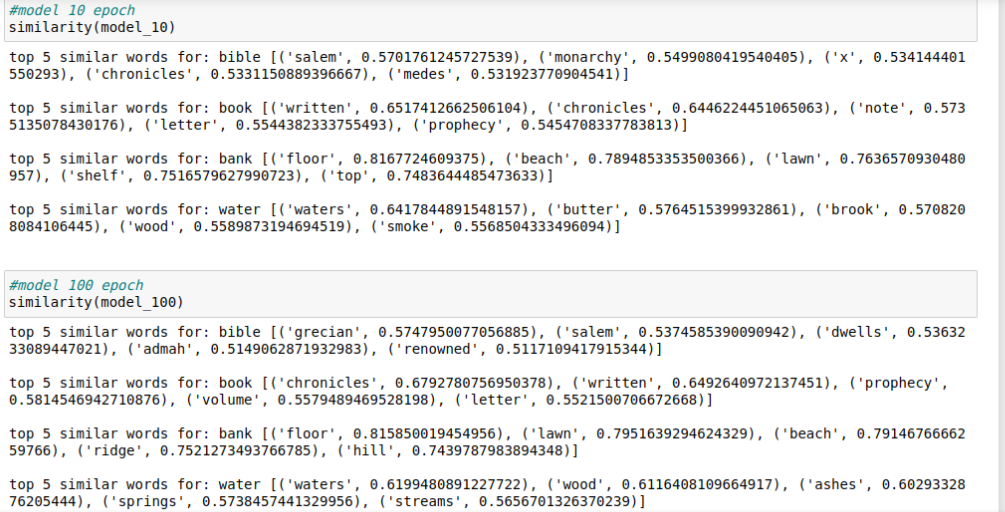
\includegraphics[width=\linewidth]{\imagesPath/lab1/images/step12_model_10_100.png}
			\end{figure}
			
            \begin{figure}[H]
				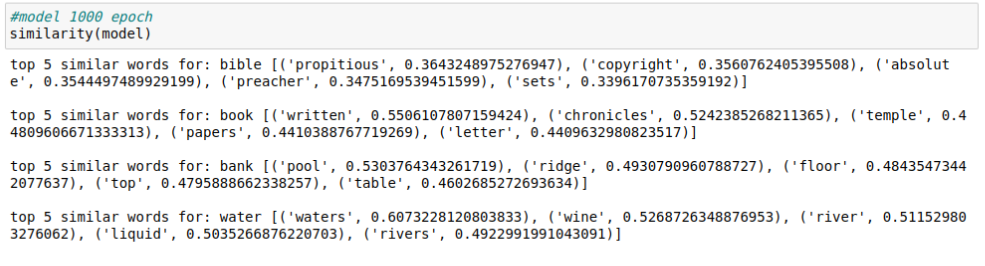
\includegraphics[width=\linewidth]{\imagesPath/lab1/images/step12_model_1000.png}
            \end{figure}
            
            \paragraph*{4)}
            	Η αύξηση των εποχών είναι μια καλή ιδέα αλλά έχει ένα τέλμα γιατί μπορεί να οδηγήσει σε over fitting. Το καλύτερο είναι να αυξήσουμε τα δεδομένα (πχ. ερώτημα ε)
        
        \subsubsection*{δ)} 
        	Ομοίως με το παραπάνω ερώτημα κάναμε το ίδιο για τις τριπλέτες λέξεων που μας δόθηκαν: 
			
			\begin{figure}[H]
				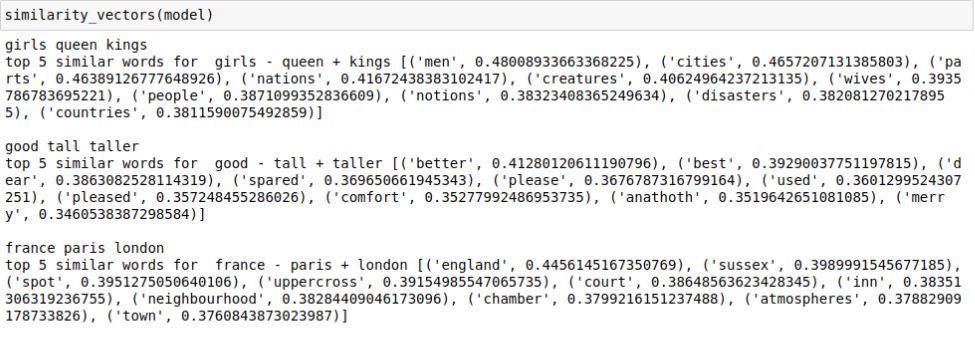
\includegraphics[width=\linewidth]{\imagesPath/lab1/images/step12_triple.png}
			\end{figure}

        \subsubsection*{ε)}
	        Κατεβάζουμε το αρχείο  και φορτώνουμε το μοντελο στην μνήμη  με limit = 250000
        
        \subsubsection*{στ, {ζ)}}
	        Έδω ακολουθούμε την ίδια διαδικασία και παρατηρούμε παρεμφερή, αλλά καλύτερα αποτελέσματα από αυτά των 1000 εποχών. Αυτό είναι λογικό γιατί περιλαμβάνει περισσότερα βιβλία και η κάθε λέξη αποτελείται από 300διάστατα διανύσματα: 
	        
        \begin{figure}[H]
        	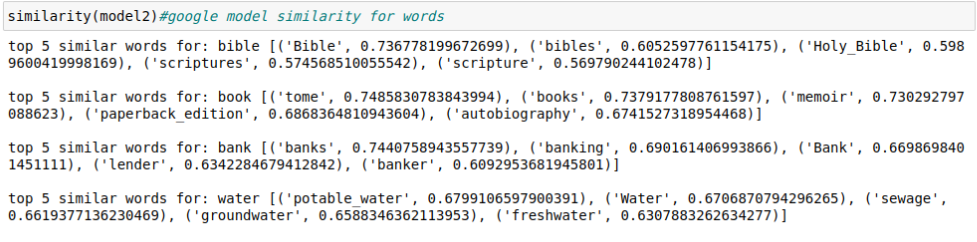
\includegraphics[width=\linewidth]{\imagesPath/lab1/images/step12_words.png}
        \end{figure}
        
        \begin{figure}[H]
        	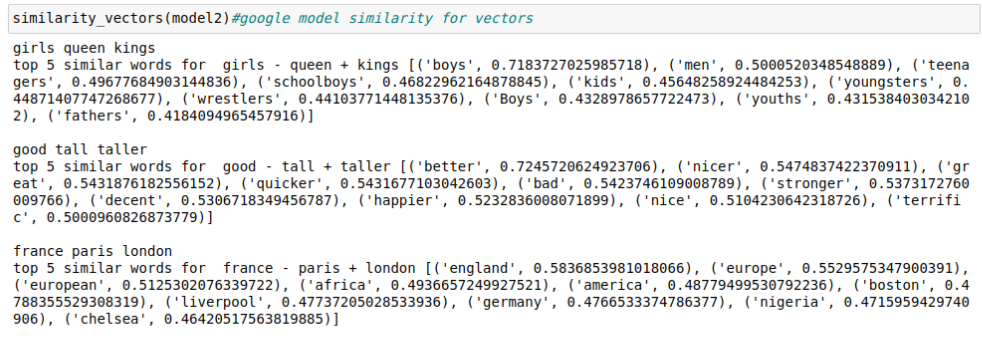
\includegraphics[width=\linewidth]{\imagesPath/lab1/images/step12_vectors.png}
        \end{figure}       
        
    \subsection*{Βήμα 13: Οπτικοποίηση των word embeddings}
        \subsubsection*{α)}
        	Εδώ πειραματιστήκαμε με το online πρόγραμμα αυτό και πραγματοποιήσαμε τις πράξεις:
        	
        	\begin{verbatim}
				France - Paris + Tokyo
				Paris - France + Japan
        	\end{verbatim}
        	
        	Παρατηρούμε ότι ο κοντινότερος γείτονας της πράξης \verb|France - Paris + Tokyo| είναι \verb|Japan| και της \verb|Paris - France + Japan| είναι \verb|Tokyo|.
        
        \begin{figure}[H]
        	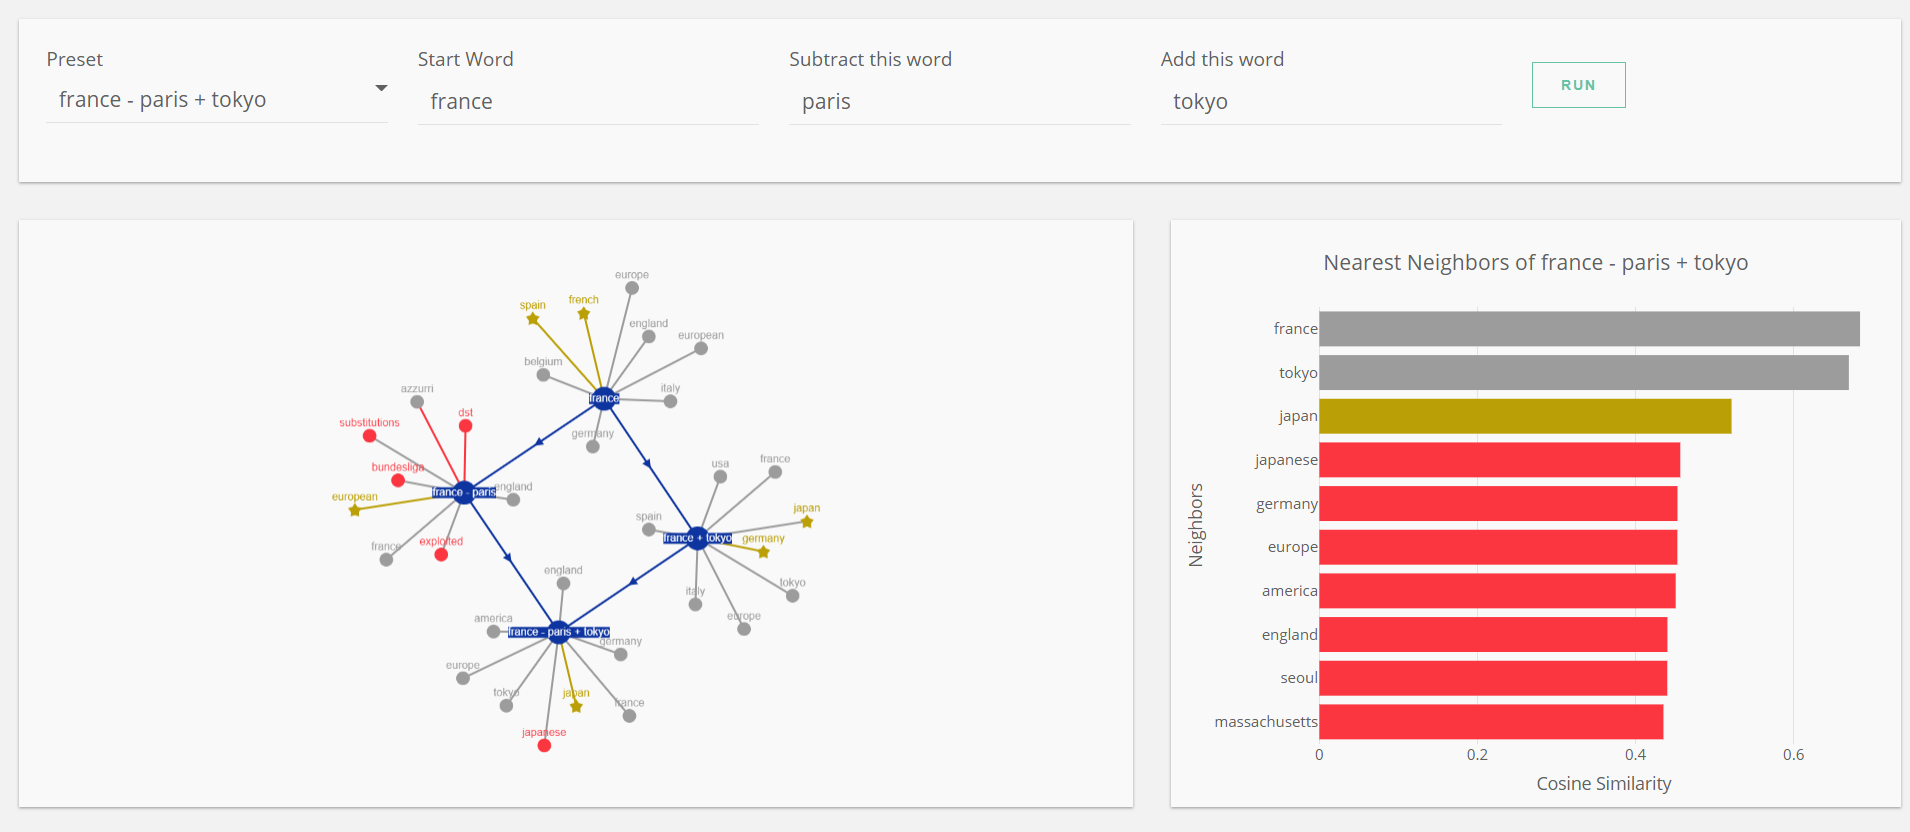
\includegraphics[width=\linewidth]{\imagesPath/lab1/images/step13_original.png}
        \end{figure}
        
        \begin{figure}[H]
        	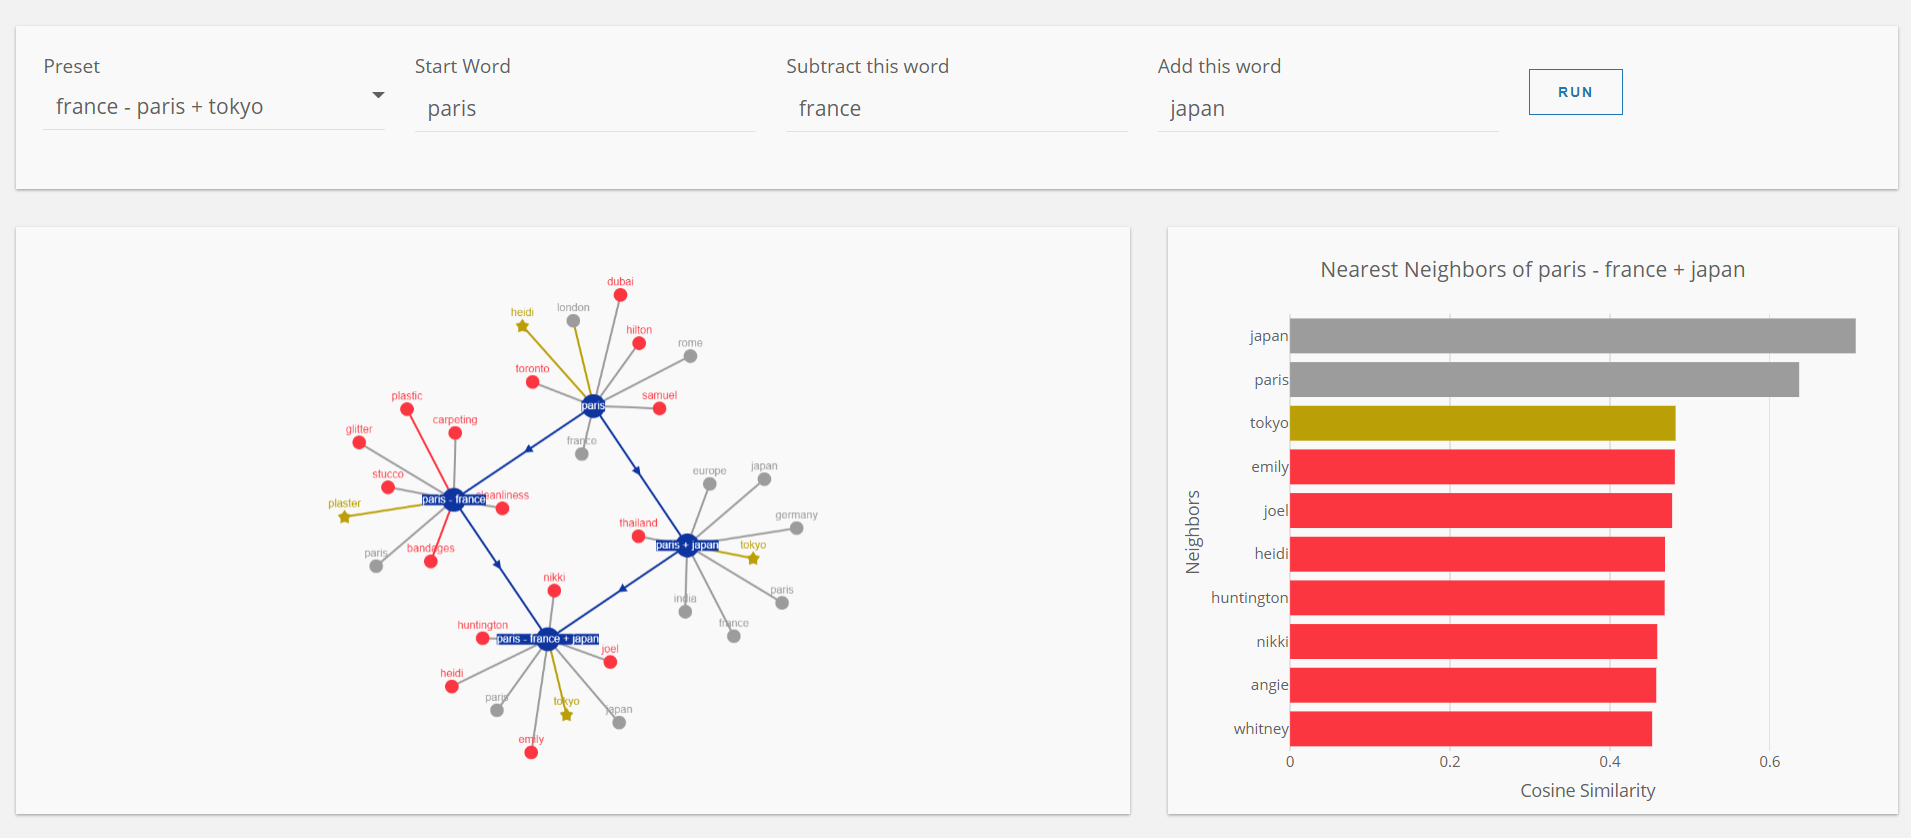
\includegraphics[width=\linewidth]{\imagesPath/lab1/images/step13_original2.png}
        \end{figure}
        
        \subsubsection*{β)}
        	Εξάγουμε το \verb|embeddings.tsv| και το \verb|metadata.tsv|.
        
        \subsubsection*{γ)}
        	Βάζουμε τα παραπάνω αρχεία στον Embedding Projector και τα οπτικοποιούμε σε 3διάστατο χώρο με τις  τεχνικές T-SNE (είναι μια non-linear μέθοδος μείωσης διαστάσεων και χρησιμοποιεί ένα t-distributed variant) και PCA (που είναι μια linear μέθοδος). Παίρνουμε τα εξής αποτελέσματα:
        	
        	\begin{itemize}
        		\item Για τον PCA:
        			\begin{itemize}
        				\item H λέξη water:
					        \begin{figure}[H]
								        	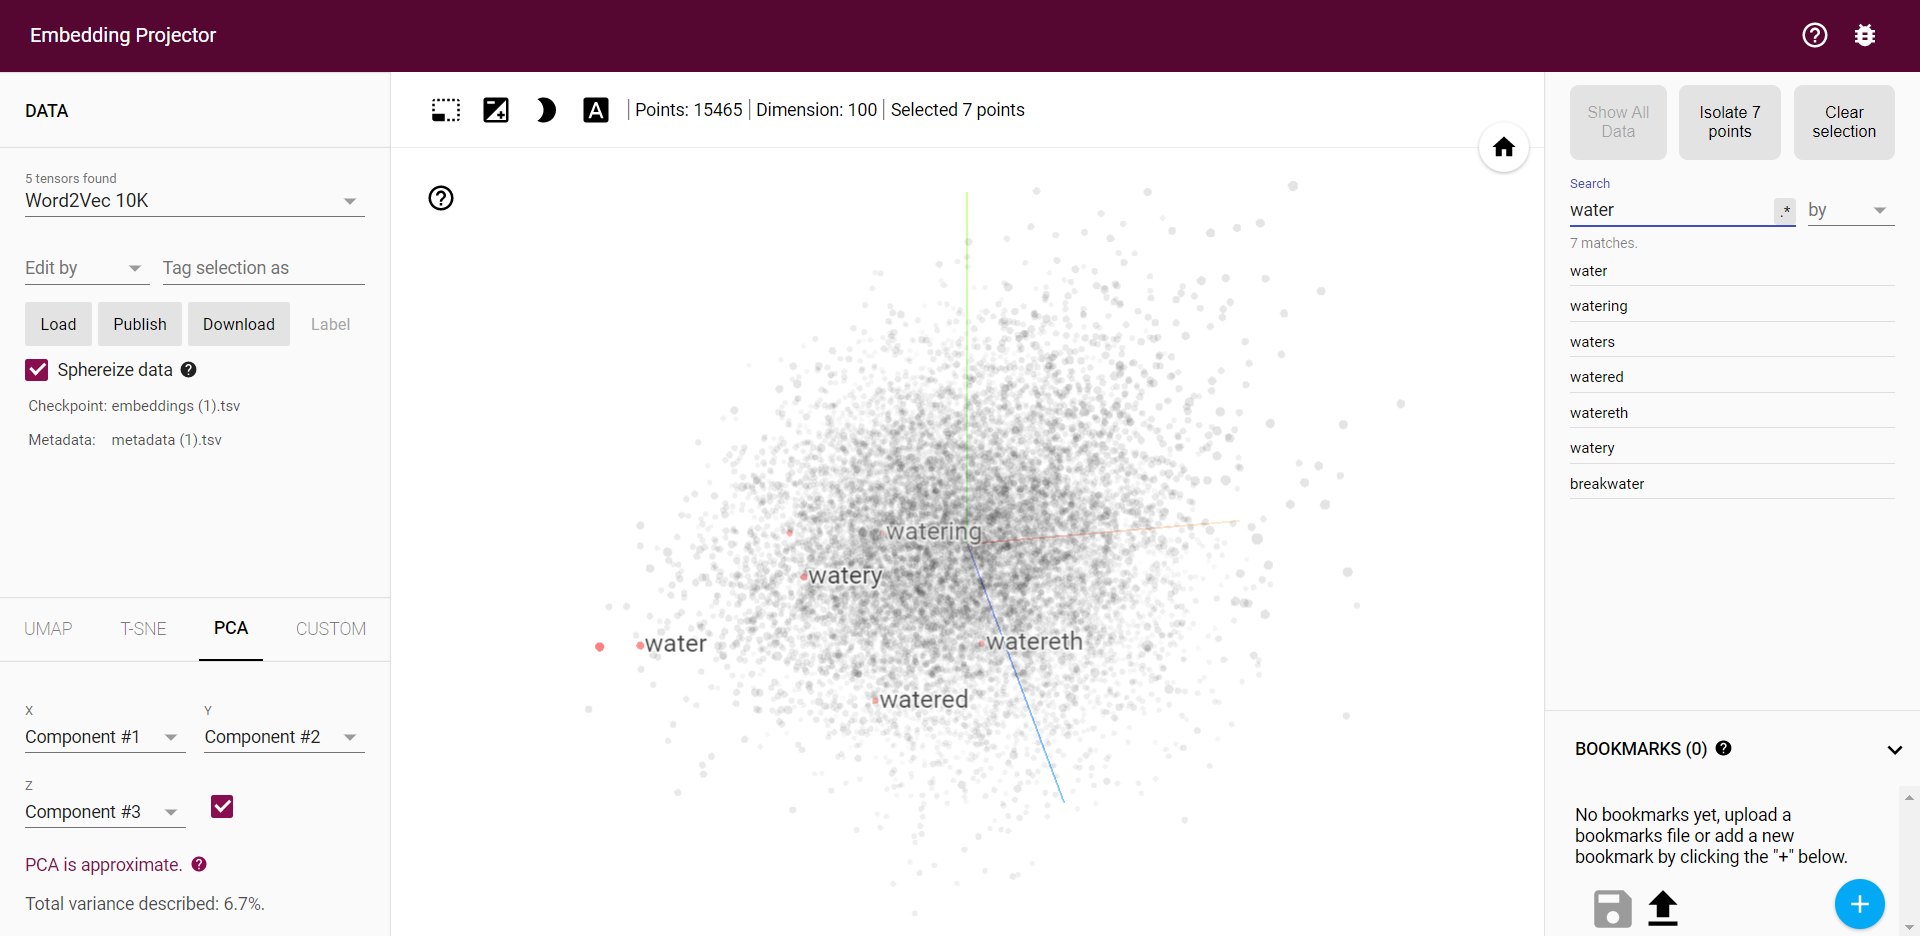
\includegraphics[width=\linewidth]{\imagesPath/lab1/images/step13_PCA_water.png}
					        \end{figure}
					       παρατηρούμε ότι είναι κοντά στην λέξη watery, watering
						\item        Η λέξη book:
					       \begin{figure}[H]
      					       	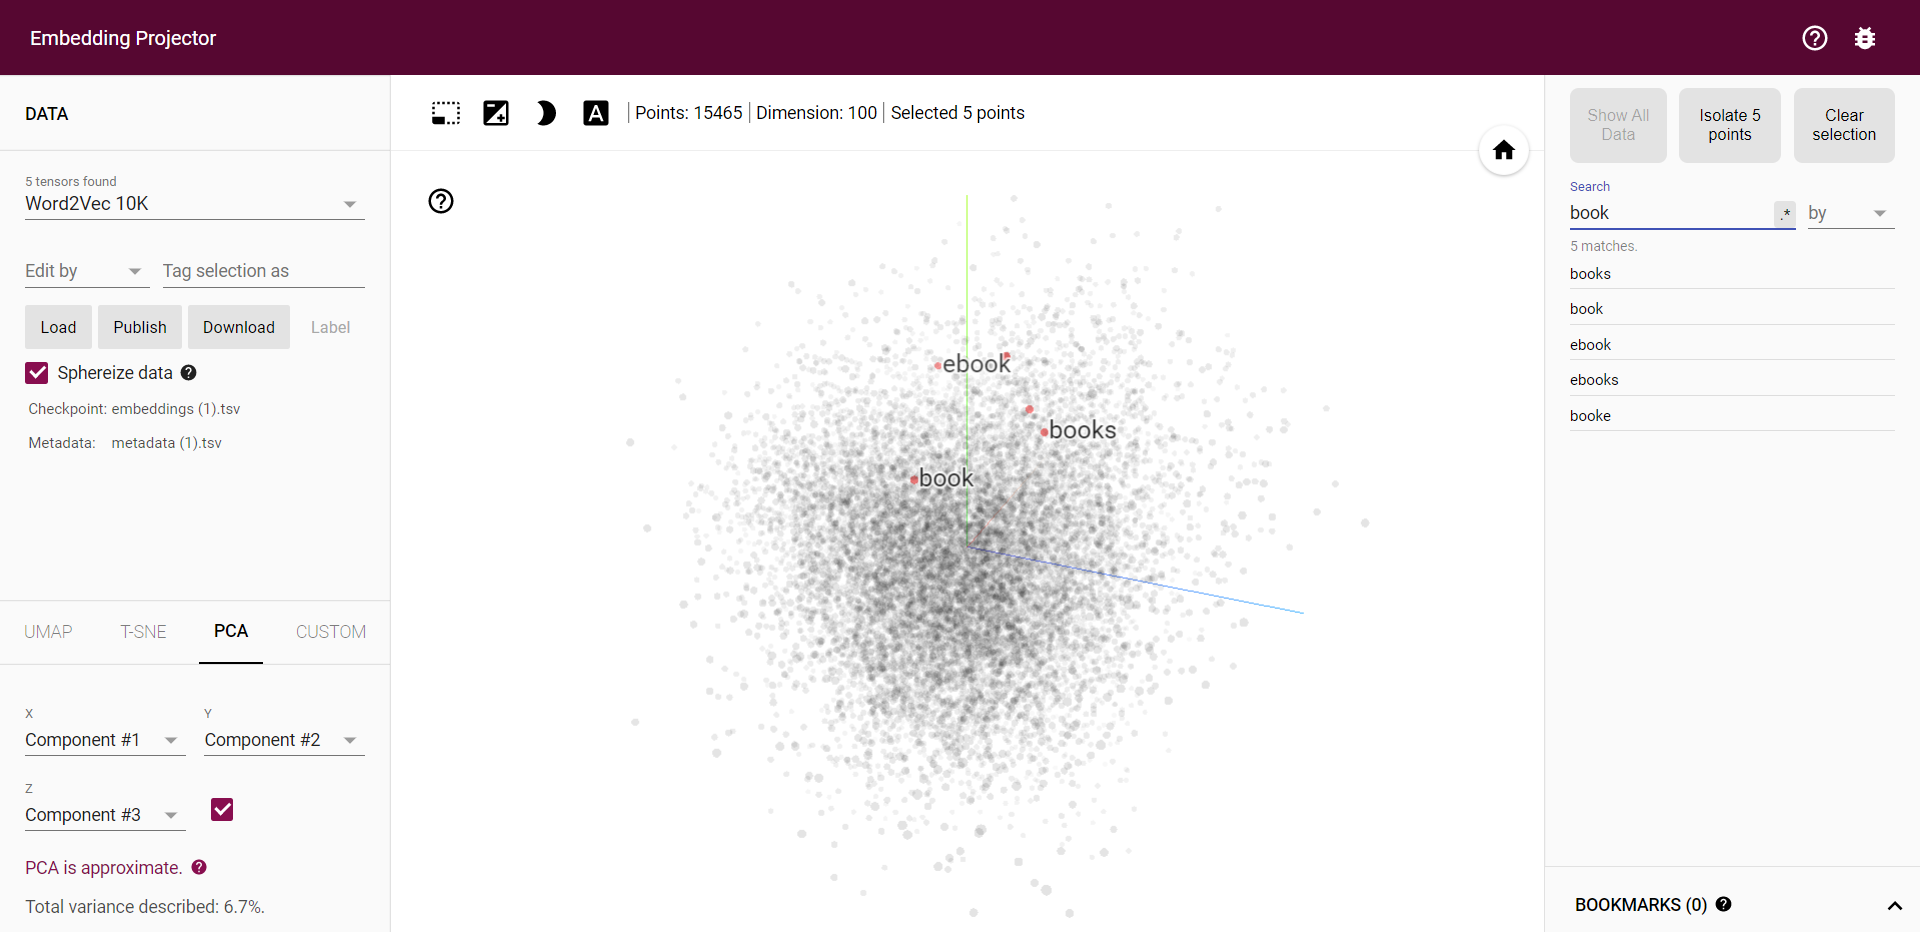
\includegraphics[width=\linewidth]{\imagesPath/lab1/images/step13_PCA_book.png}
					       \end{figure}
					       
					       παρατηρούμε ότι είναι κοντά στη λέξη ebook, books.
        			\end{itemize}
        		\item Για τον T-SNE:
        			\begin{itemize}
        				\item H λέξη water:
			    		        \begin{figure}[H]
			    				    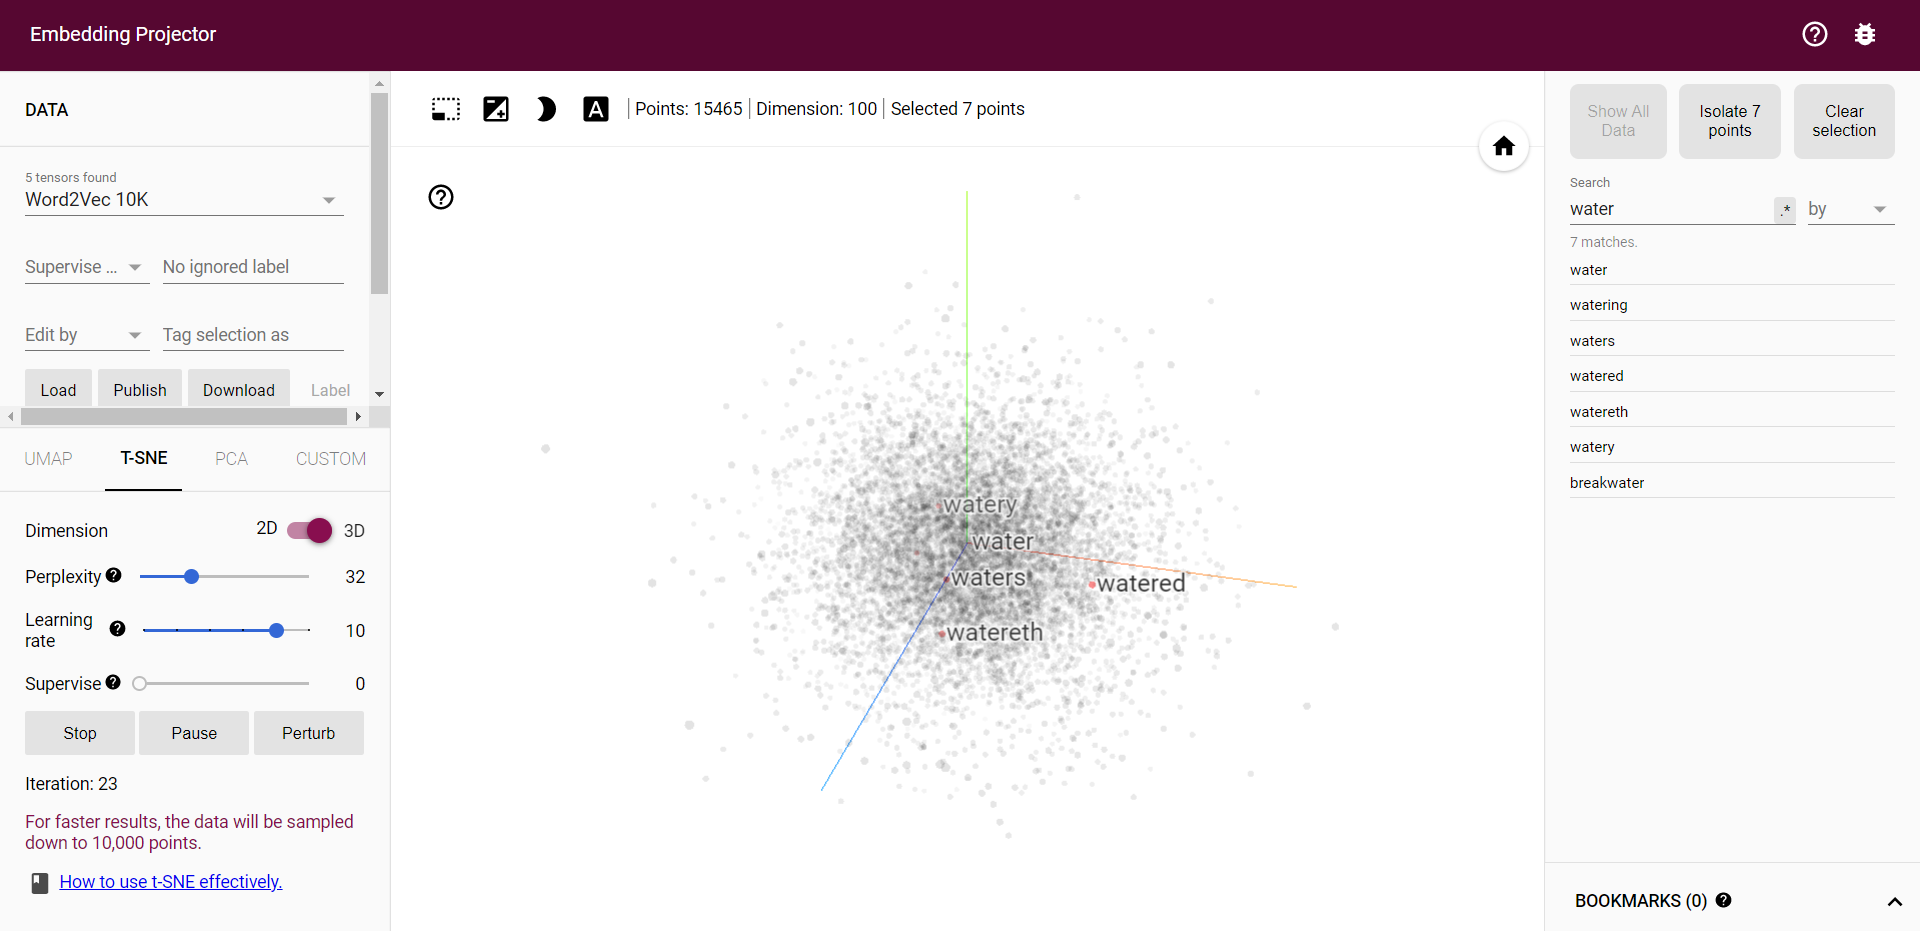
\includegraphics[width=\linewidth]{\imagesPath/lab1/images/step13_TSNE_water.png}
			    		        \end{figure}
        				 \item Η λέξη book:
					           \begin{figure}[H]
					           		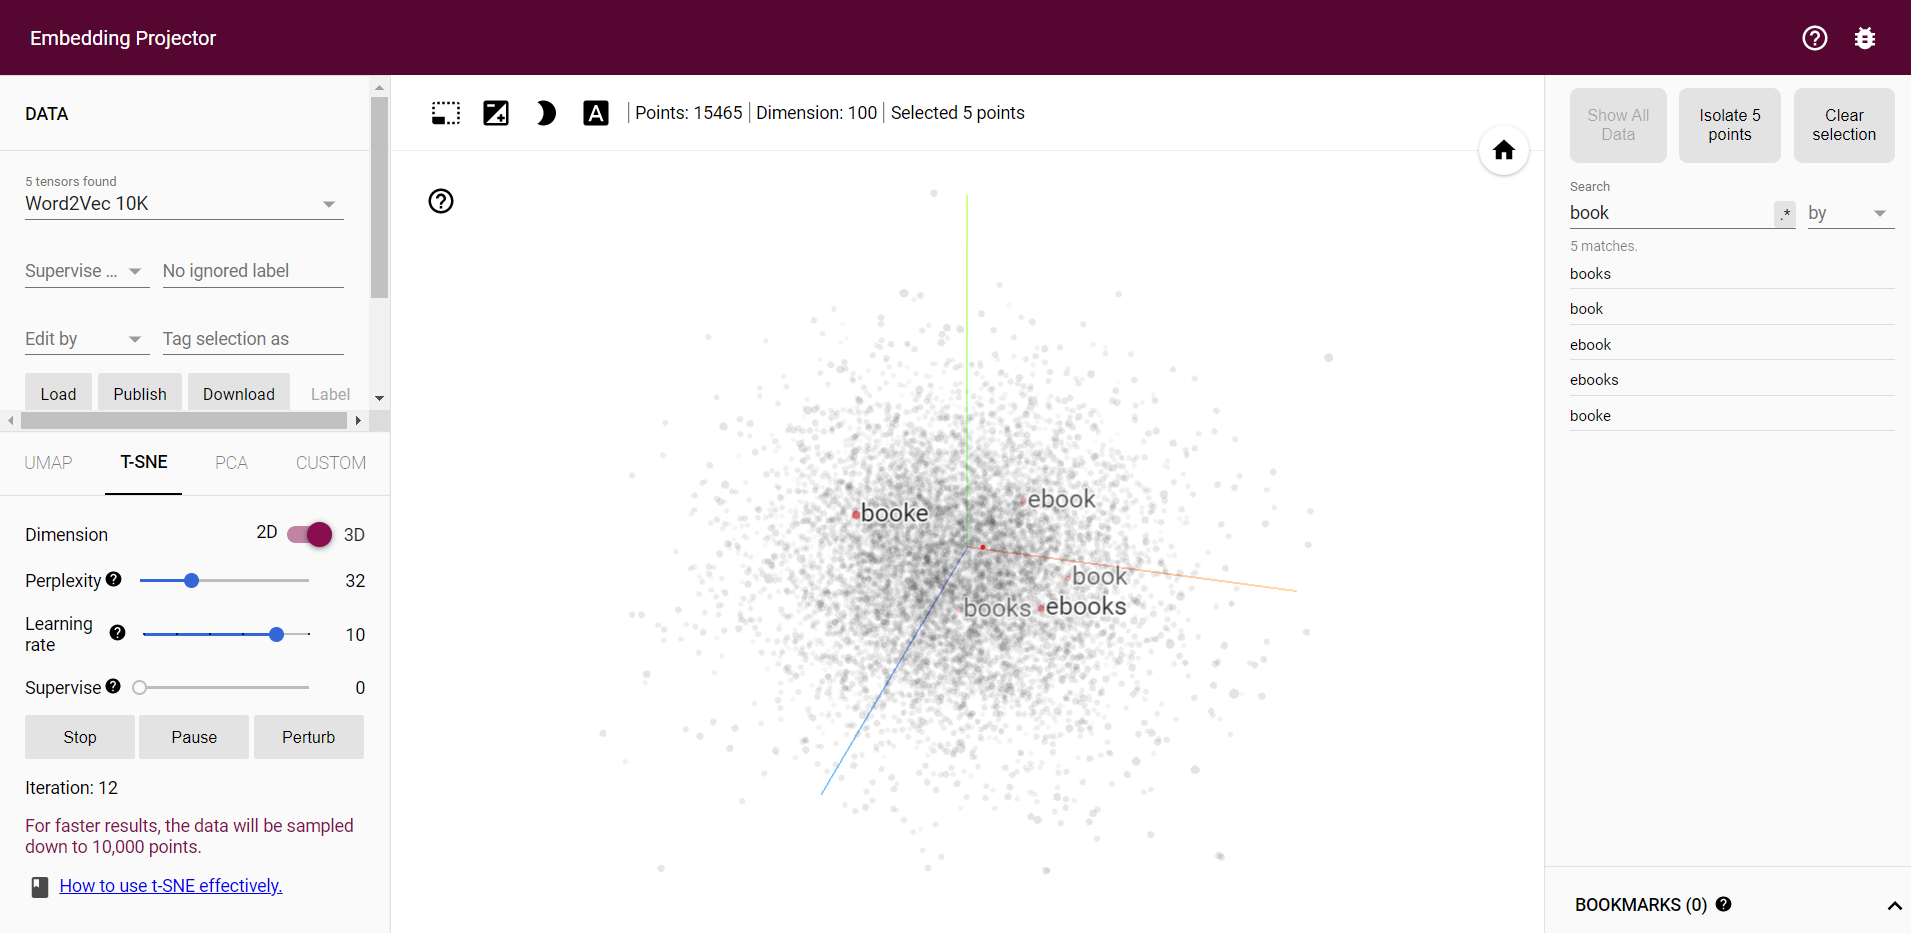
\includegraphics[width=\linewidth]{\imagesPath/lab1/images/step13_TSNE_book.png}
					           \end{figure}
        			\end{itemize}			
        	\end{itemize}

    \subsection*{Βήμα 14: Ανάλυση συναισθήματος με word2vec embeddings}
        \subsubsection*{α)}
        	Αρχικά κατεβάσαμε τα δεδομένα που ζητούνται.
        \subsubsection*{β)}
        	Yλοποιήσαμε τον κώδικα \verb|w2v_sentiment_analysis.py| και χρησιμοποιήσαμε το μοντέλο που εκπαιδεύσαμε για την εξαγωγή τον embeddings των θετικών και αρνητικών σχολίων από το dataset. Mέσω της μεθόδου Neural Bag of Words  υπολογίσαμε τα embeddings των προτάσεων ως μέσο όρο των word embeddings των λέξεων που τις αποτελούν ως 100διάστατα διανύσματα για κάθε πρόταση.
        \subsubsection*{γ)}
        	Στην συνέχεια εκπαιδεύσαμε το Logistic Regression Model ώστε να προβλέπει αν μια πρόταση είναι θετική η αρνητική με ποσοστό ακρίβειας 74.14\%
        \subsubsection*{δ)}
        	Επαναλάβαμε το παραπάνω βήμα χρησιμοποιώντας τα embeddings από το μοντέλο της Google με ποσοστό 83.2\%.
\end{document}